\documentclass[a4paper,11pt,fleqn]{article}

\usepackage[left=1cm,right=1cm,top=0.5cm,bottom=2cm]{geometry}

\usepackage{bfcours}
\usepackage{bfcours-fonts}
%\usepackage{bfcours-fonts-dys}
\pgfplotsset{compat=1.18}
\def\rdifficulty{1}
\setrdexo{%left skip=1cm,
display exotitle,
exo header = tcolorbox,
%display tags,
skin = bouyachakka,
lower ={box=crep},
display score,
display level,
save lower,
score=\points,
level=\rdifficulty,
overlay={\node[inner sep=0pt,
anchor=west,rotate=90, yshift=0.3cm]%,xshift=-3em], yshift=0.45cm
at (frame.south west) {\thetags[0]} ;}
]%obligatoire
}
\setrdcrep{seyes, correction=true, correction color=monrose, correction font = \large\bfseries}

\newcommand{\tikzinclude}[1]{%
    \stepcounter{tikzfigcounter}%
    \csname tikzfig#1\endcsname
}
\newcommand{\tikzfigTnVi}{
\begin{tikzpicture}[line cap=round,line join=round,>=triangle 45,x=1.0cm,y=1.0cm,scale=0.6]
\begin{axis}[
x=1.0cm,y=1.0cm,
axis lines=middle,
ymajorgrids=true,
xmajorgrids=true,
xmin=-1.5,
xmax=3.5,
ymin=-3.2,
ymax=3.2,
xtick={-1.0,0.0,...,3.0},
ytick={-3.0,-2.0,...,3.0},]
\clip(-1.5,-3.2) rectangle (3.5,3.2);
\draw[line width=2.pt,color=blue,smooth,samples=100,domain=-1.5:3.5] plot(\x,{-0.6*((\x)-1.0)^(2.0)+2.0});
\begin{scriptsize}
\draw[color=blue] (-1,1) node {\large{$\mathcal{C}_f$}};
\end{scriptsize}
\end{axis}
\end{tikzpicture}
}

\newcommand{\tikzfigXWyE}{
\begin{tikzpicture}[line cap=round,line join=round,>=triangle 45,x=1.0cm,y=1.0cm,scale=0.6]
\begin{axis}[
x=1.0cm,y=1.0cm,
axis lines=middle,
ymajorgrids=true,
xmajorgrids=true,
xmin=-1.5,
xmax=3.5,
ymin=-3.2,
ymax=3.2,
xtick={-1.0,0.0,...,3.0},
ytick={-3.0,-2.0,...,3.0},]
\clip(-1.5,-3.2) rectangle (3.5,3.2);
\draw[line width=2.pt,color=blue,smooth,samples=100,domain=-1.5:3.5] plot(\x,{0.5*((\x)-2.0)^(2.0)-3.0});
\begin{scriptsize}
\draw[color=blue] (-1,2.5) node {\large{$\mathcal{C}_g$}};
\end{scriptsize}
\end{axis}
\end{tikzpicture}
}

\newcommand{\tikzfigbxUA}{
\begin{tikzpicture}[line cap=round,line join=round,>=triangle 45,x=1.0cm,y=1.0cm,scale=0.6]
\begin{axis}[
x=1.0cm,y=1.0cm,
axis lines=middle,
ymajorgrids=true,
xmajorgrids=true,
xmin=-1.5,
xmax=3.5,
ymin=-3.2,
ymax=3.2,
xtick={-1.0,0.0,...,3.0},
ytick={-3.0,-2.0,...,3.0},]
\clip(-1.5,-3.2) rectangle (3.5,3.2);
\draw[line width=2.pt,color=blue,smooth,samples=100,domain=-1.5:3.5] plot(\x,{0-0.3*((\x)-1.0)^(2.0)-1.0});
\begin{scriptsize}
\draw[color=blue] (2.5,-1) node {\large{$\mathcal{C}_h$}};
\end{scriptsize}
\end{axis}
\end{tikzpicture}
}

\newcommand{\tikzfigzaPA}{
\begin{tikzpicture}[line cap=round,line join=round,>=triangle 45,x=1.0cm,y=1.0cm,scale=0.6]
\begin{axis}[
x=1.0cm,y=1.0cm,
axis lines=middle,
ymajorgrids=true,
xmajorgrids=true,
xmin=-1.5,
xmax=3.5,
ymin=-3.2,
ymax=3.2,
xtick={-1.0,0.0,...,3.0},
ytick={-3.0,-2.0,...,3.0},]
\clip(-1.5,-3.2) rectangle (3.5,3.2);
\draw[line width=2.pt,color=blue,smooth,samples=100,domain=-1.5:3.5] plot(\x,{0-1*((\x)+0.0)^(2.0)+2.0});
\begin{scriptsize}
\draw[color=blue] (-1,2.5) node {\large{$\mathcal{C}_i$}};
\end{scriptsize}
\end{axis}
\end{tikzpicture}
}

\newcommand{\tikzfigmWht}{
\begin{tikzpicture}[line cap=round,line join=round,>=triangle 45,x=1.0cm,y=1.0cm,scale=0.8]
\clip(2.5,0.5) rectangle (9.5,5.5);
\fill[line width=2.pt,color=ffffff,fill=ffffff,fill opacity=1.0] (3.,5.) -- (9.,5.) -- (9.,1.) -- (3.,1.) -- cycle;
\fill[line width=0.pt,color=ffqqqq,fill=ffqqqq,fill opacity=1.0] (3.,5.) -- (3.,3.5) -- (4.5,3.5) -- (4.5,5.) -- cycle;
\fill[line width=0.pt,color=ffqqqq,fill=ffqqqq,fill opacity=1.0] (3.,1.) -- (3.,2.5) -- (4.5,2.5) -- (4.5,1.) -- cycle;
\fill[line width=0.pt,color=ffqqqq,fill=ffqqqq,fill opacity=1.0] (5.5,1.) -- (5.5,2.5) -- (9.,2.5) -- (9.,1.) -- cycle;
\fill[line width=0.pt,color=ffqqqq,fill=ffqqqq,fill opacity=1.0] (5.5,5.) -- (5.5,3.5) -- (9.,3.5) -- (9.,5.) -- cycle;
\draw [line width=2.pt] (3.,5.)-- (9.,5.);
\draw [line width=2.pt] (9.,5.)-- (9.,1.);
\draw [line width=2.pt] (9.,1.)-- (3.,1.);
\draw [line width=2.pt] (3.,1.)-- (3.,5.);
\end{tikzpicture}
}

\newcommand{\tikzfigFuya}{
\begin{tikzpicture}[line cap=round,line join=round,>=triangle 45,x=1.0cm,y=1.0cm,scale=1]
\clip(-0.1,-0.1) rectangle (4.1,4.1);
\fill[line width=1.pt,color=blue,fill=blue!30,fill opacity=1] (0,0) -- (3.,0.) -- (0.,1.) -- cycle;
\fill[line width=1.pt,color=red,fill=blue!30,fill opacity=1] (4,0) -- (4,3) -- (3,0) -- cycle;
\fill[line width=1.pt,color=blue,fill=blue!30,fill opacity=1] (4,4) -- (1,4) -- (4,3) -- cycle;
\fill[line width=1.pt,color=blue,fill=blue!30,fill opacity=1] (0,4) -- (0,1) -- (1,4) -- cycle;
\draw [line width=1.pt,color=blue] (0,0)-- (4,0);
\draw [line width=1.pt,color=blue] (4,0)-- (4,4);
\draw [line width=1.pt,color=blue] (4,4.)-- (0,4);
\draw [line width=1.pt,color=blue] (0,4)-- (0,0);
\draw [line width=1.pt,color=blue] (0,1)-- (3,0);
\draw [line width=1.pt,color=blue] (3,0)-- (4,3);
\draw [line width=1.pt,color=blue] (4,3)-- (1,4);
\draw [line width=1.pt,color=blue] (1,4)-- (0,1);
\end{tikzpicture}
}



\hypersetup{
    pdfauthor={R.Deschamps},
    pdfsubject={},
    pdfkeywords={},
    pdfproducer={LuaLaTeX},
    pdfcreator={Boum Factory}
}
% Activer ou désactiver l'affichage des boîtes pour les points
%\displayitempointsfalse % Ne pas afficher les boîtes
\displayitempointstrue % Afficher les boîtes
\renewcommand{\boldsymbol}[1]{#1}


\newcommand{\intervalle}[2]{\CrochetG #1 ; #2\,\,\CrochetD}
\begin{document}

\setcounter{pagecounter}{0}
\setcounter{ExoMA}{0}

\def\points{\phantom{AAA}}
\def\difficulty{\phantom{AAA}}
\chapitre[
    $\mathbf{1^{\text{ère}}}$% : $\mathbf{6^{\text{ème}}}$,$\mathbf{5^{\text{ème}}}$,$\mathbf{4^{\text{ème}}}$,$\mathbf{3^{\text{ème}}}$,$\mathbf{2^{\text{nde}}}$,$\mathbf{1^{\text{ère}}}$,$\mathbf{T^{\text{Le}}}$,
    ]{
    Aires et polynômes de degré 2% : ,Equations
    }{
    Lycée% : Collège,Lycée
    }{
    Camille Claudel% : Othe et Vanne,Amadis Jamyn,Eugène Belgrand
    }{
    % : 10},15},30},55}%}
    }{
    Complément :
    }

\setrdcrep{seyes, correction=true, correction color=monrose, correction font = \large\bfseries}


\begin{EXO}{Problème ouvert}{}
    \vspace{-0.5cm}\begin{flushright}\textit{(source: académie Aix-Marseille)}\end{flushright}
    \vspace{-0.4cm}\tcbitempoint{20} Le laboratoire d'une aciérie étudie la dilatation d'un acier fabriqué par l'entreprise.

Les mesures effectuées donnent les résultats suivants pour une tige d'acier :
\begin{center}
\begin{tcbtab}{|c|c|c|c|c|c|}
Température en $^\circ$C & 0 & 50 & 100 & 200 & 400 \\\hline
Longueur en cm & \num{50} & \num{50.03} & \num{50.06} & \num{50.12} & \num{50.24} \\\hline
\end{tcbtab}
\end{center}

\begin{tcbenumerate}
\tcbitem A \acc{quelle température} faut-il porter la tige pour que sa longueur soit égale à \num{50,15}cm ?


\tcbitem La température la plus basse que l'on peut atteindre est appelé le zéro absolue. Sa température est de \num{-273.15}$^\circ$C.

\acc{Est-il possible} de réduire la taille de la tige d'acier d'\acc{un centième} de sa taille initiale ?
\end{tcbenumerate}
\exocorrection
\begin{MultiColonnes}{2}
    \tcbitem L'\acc{allongement} $A$ de la tige d'acier semble être \acc{proportionnel} à la \acc{température} de la tige. 
    
    En effet : 
    \tcbitem[halign=center] \begin{tcbtab}{c|c|c|c|c}
\acc{Température} en $^\circ$C &50 & 100 & 200 & 400 \\\hline
Longueur en cm & \num{50.03} & \num{50.06} & \num{50.12} & \num{50.24} \\\hline
\acc{Allongement} en cm & \num{0.03} & \num{0.06} & \num{0.12} & \num{0.24} \\
\end{tcbtab}
\end{MultiColonnes}
On vérifie que les lignes Température et Allongement sont proportionnelles en calculant les rapports $\dfrac{A}{T}$ dans chaque colonne : 
\vspace{-0.35cm}\begin{multicols}{2}
\foreach \x/\y in {50/0.03 , 100/0.06 , 200/0.12 , 400/0.24 } {
    $\dfrac{\num{\y}}{\x} = \displaystyle{\Simplification{\fpeval{\y*100}}{\fpeval{\x*100}}}=\num{\fpeval{\y/\x}}$ \\ \phantom{a} \\
}
\end{multicols}

\vspace{-1cm}Le \acc{coefficient de proportionnalité} est $\num{0.0006}=\num{6d-4}$ et on en déduit : 

$A = \num{6d-4} \times T$. 

On peut observer le lien suivant : L = \encadrer[defi]{Longueur initiale} + \encadrer[blue]{Allongement}

\begin{tcolorbox}[
    colback=green!10,
    colframe=green!50!black,
    title={\faCalculator\space Modélisation mathématique}
]
À partir de ces observations et calculs, on peut déterminer l'expression de la \acc{fonction} donnant la \acc{longueur} $L$ de la tige en fonction de la \acc{température} $T \in \intervalle[ff]{0}{400}$:
\begin{center}
$L:T\mapsto \underbrace{50}_{L_0} + \underbrace{\num{6d-4}T}_{\text{Allongement}}$
\end{center}

Puisque l'expression est définie sur $\R$, il est \acc{naturel} d'étendre son domaine de définition pour 

$T\in \intervalle[ff]{\num{-273.15}}{400}$ ce qui permet de répondre aux deux questions de façon raisonnable. 
\end{tcolorbox}

\textbf{\large Graphique des données expérimentales}

\begin{center}
\begin{tikzpicture}[scale=0.9]
    % Axes
    \draw[thick,->] (-0.5,0) -- (11,0) node[right] {$T$ ($^\circ$C)};
    \draw[thick,->] (0,-0.5) -- (0,9) node[above] {$L$ (cm)};

    % Graduations axe x
    \foreach \x/\xtext in {0/0, 2/100, 4/200, 6/300, 8/400, 10/500} {
        \draw (\x,0.1) -- (\x,-0.1) node[below] {\num{\xtext}};
    }

    % Graduations axe y
    \foreach \y/\ytext in {0/50.00, 2/50.06, 4/50.12, 6/50.18, 6.67/50.20, 8/50.24} {
        \draw (0.1,\y) -- (-0.1,\y) node[left] {\num{\ytext}};
    }

    % Points expérimentaux
    \coordinate (A) at (0,0);
    \coordinate (B) at (1,1);
    \coordinate (C) at (2,2);
    \coordinate (D) at (4,4);
    \coordinate (E) at (8,8);

    % Tracer les points
    \foreach \point/\x/\y in {A/0/0,B/1/1,C/2/2,D/4/4,E/8/8} {
        \fill[red] (\point) circle (2pt);
        \draw[gray!70!black,dashed] (\point) -- (\x,0) node[below] {};
        \draw[gray!70!black,dashed] (\point) -- (0,\y) node[left] {};
    }

    % Points avec leurs coordonnées
    %\node[above right] at (A) {$(0, 50.00)$};
    %\node[above right] at (B) {$(50, 50.03)$};
    %\node[above right] at (C) {$(100, 50.06)$};
    %\node[above right] at (D) {$(200, 50.12)$};
    %\node[above right] at (E) {$(400, 50.24)$};

    % Régression linéaire
    \draw[blue,thick,dashed] (-1.5,-1.5) -- (8.5,8.5) node[right] {$L(T) = 50 + 6 \times 10^{-4} T$};

    % Point recherché pour question 1
    \coordinate (F) at (5,5);
    \fill[green!70!black] (F) circle (2pt);
    \draw[green!70!black,dashed] (F) -- (5,0) node[below] {$250$};
    \draw[green!70!black,dashed] (F) -- (0,5) node[left] {$\num{50.15}$};
    \node[above right,green!70!black,yshift=-10pt] at (F) {Solution Q1};
\end{tikzpicture}
\end{center}

\begin{tcbenumerate}[2]
\tcbitem Température pour $L = \num{50.15}$ cm
\begin{tcolorbox}[
    colback=blue!10,
    colframe=blue!50!black,
    title={\faThermometerHalf\space Résolution :}
]
Nous cherchons $T$ tel que $L(T) = \num{50.15}$ cm.
\begin{align*}
50 + 6 \times 10^{-4} T &= \num{50.15}\\[0.15cm]
6 \times 10^{-4} T &= \num{0.15}\\[0.15cm]
T &= \frac{\num{0.15}}{6 \times 10^{-4}}\\[0.15cm]
T &= \frac{\num{0.15} \times 10^{4}}{6}\\[0.15cm]
T &= \frac{1500}{6}\\[0.15cm]
T &= \boxed{250 ^\circ\text{C}}
\end{align*}

\textbf{Vérification :} $L(250) = 50 + 6 \times 10^{-4} \times 250 = 50 + \num{0.15} = \num{50.15}$ 

\bcoeil On pouvait aussi résoudre \acc{graphiquement} cette question ( voir graphique précédent ).
\end{tcolorbox}

\tcbitem Réduction d'un centième de la taille initiale

\begin{tcolorbox}[
    colback=red!10,
    colframe=red!50!black,
    title={\faSnowflake\space Analyse de la contraction thermique :}
]
Une réduction d'un centième signifie que la tige devrait mesurer : 

$L_{\text{reduit}} = L_{\text{initial}} - \frac{L_{\text{initial}}}{100} = 50 - 0.5 = \num{49.5}$ cm

    Cherchons la température nécessaire :
\begin{align*}
50 + 6 \times 10^{-4} T &= \num{49.5}\\[0.15cm]
6 \times 10^{-4} T &= -\num{0.5}\\[0.15cm]
T &= \frac{-\num{0.5}}{6 \times 10^{-4}}\\[0.15cm]
T &= -\frac{5000}{6}\\[0.15cm]
T &\approx \boxed{-\num{833.33} ^\circ\text{C}}
\end{align*}

Or, Le zéro absolu est à $-\num{273.15}$ $^\circ$C et aucune température ne peut descendre en dessous. 

\textbf{Conclusion :} Cette température étant impossible à atteindre, on ne peut pas réduire la tige d'un centième de sa taille initiale.

\end{tcolorbox}
\end{tcbenumerate}

\vspace{0.5cm}

\begin{tcolorbox}[
    colback=purple!10,
    colframe=purple!50!black,
    title={\faGraduationCap\space Remarques :}
]
\begin{tcbenumerate}
    \tcbitem[colback=purple!10] \textbf{Modèle affine :} La dilatation de cet acier peut être \acc{modélisé} par une fonction affine $L(T) = 50 + \num{6d-4}T$

    Dans le cadre de ce devoir et d'après les données disponibles, \acc{on a supposé que} le modèle affine suggéré par les données est valable pour $T>-273{,}15^\circ$.

    Ce n'est pas nécessairement vrai, mais cela \acc{suffit} à répondre à la question posée. 

    En effet il y a peu de chances que la contraction thermique se produise plus facilement au fur et à mesure que la température diminue. 
    \tcbitem[colback=purple!10] \textbf{Contraction maximale :} À $T = -273.15$ $^\circ$C, $L \approx \num{49.836}$ cm , ce qui correspond à une contraction maximale de seulement $0{,}033\%$ de la longueur initiale.
    \tcbitem[colback=purple!10] En l'absence d'informations supplémentaires, le problème reste ouvert. 

    En effet, nos conlusions sont vraies dans le cadre de notre modèle et une simple hypothèse supplémentaire peut tout changer : par exemple qu'en est-il si la pression varie également ?
\end{tcbenumerate}
\end{tcolorbox}

\begin{tcbtab}[Barème pour les traces de recherche]{|p{13cm}|c|}
\textbf{Critère} & \textbf{Points} \\\hline\hline
Formulation tableau de proportionnalité ou lien affine. & /2 \\\hline
Calculs de vérification (ou partiel) & /1 \\\hline
Lien avec l'expression de la fonction ou avec le graphique. & /2 \\\hline
Modélisation par une fonction affine : explicitation par l'élève. & /2 \\\hline\hline
\textbf{Total} & \textbf{/7} \\\hline
\end{tcbtab}

\vspace{0.5cm}

\begin{tcbtab}[Barème pour la question 1]{|p{13cm}|c|}
\textbf{Critère} & \textbf{Points} \\\hline\hline
Expliquer le lien entre la question posée et le modèle déterminé. & /1 \\\hline
Trouver l'équation à résoudre pour répondre à la question 1. Ou mise en lien avec le graphique. & /2 \\\hline
Résoudre cette équation ou la résoudre graphiquement (traits de construction apparents). Pour obtenir tous les points l'élève doit avoir mentionné ou contourné (par du papier millimétré par exemple) la légère imprécision de la méthode, mais qui permet tout de même de conclure. & /2 \\\hline
Conclure & /1 \\\hline\hline
\textbf{Total} & \textbf{/6} \\\hline
\end{tcbtab}

\vspace{0.5cm}

\begin{tcbtab}[Barème pour la question 2]{|p{13cm}|c|}
\textbf{Critère} & \textbf{Points} \\\hline\hline
Expliquer le lien entre la question posée et le modèle déterminé. & /1 \\\hline
Trouver l'équation à résoudre & /2 \\\hline
Résoudre l'équation & /2 \\\hline
Conclure & /2 \\\hline\hline
\textbf{Total} & \textbf{/7} \\\hline
\end{tcbtab}


\acc{Remarques pour la question 1 : } 

\begin{itemize}
    \item Le lien entre la température et la longueur est \acc{affine}. Il était attendu que l'élève le mentionne. 
    \item Il était attendu que des calculs soient présents pour les traces de recherche.
\end{itemize}

\acc{Remarques pour la question 2 : } 

\begin{itemize}
    \item La méthode graphique est toujours possible pour la question 2 mais plus compliquée à mettre en \oe uvre. L'élève recevra tous les points s'il justifie comme dans la première question.
    \item Dans la question 2, le calcul de la longueur à $T=\num{-273.15}^\circ$ ne suffit pas : il faut en plus préciser que la fonction étant croissante, la longueur voulue ne peut effectivement être atteinte pour $T>\num{-273.15}^\circ$.
    \item Une autre stratégie plus efficace est de calculer directement la température à atteindre pour obtenir la longueur souhaitée. Cela permettait de ne pas justifier que la fonction $L(T)$ est croissante. 
\end{itemize}

\end{EXO}
% : 
\begin{EXO}{Problème ouvert}{}
    \vspace{-0.5cm}\begin{flushright}\textit{(source: académie Aix-Marseille)}\end{flushright}
    \vspace{-0.4cm}\tcbitempoint{20} Le laboratoire d'une aciérie étudie la dilatation d'un acier fabriqué par l'entreprise.

Les mesures effectuées donnent les résultats suivants pour une tige d'acier :
\begin{center}
\begin{tcbtab}{|c|c|c|c|c|c|}
Température en $^\circ$C & 0 & 50 & 100 & 200 & 400 \\\hline
Longueur en cm & \num{50} & \num{50.03} & \num{50.06} & \num{50.12} & \num{50.24} \\\hline
\end{tcbtab}
\end{center}

\begin{tcbenumerate}
\tcbitem A \acc{quelle température} faut-il porter la tige pour que sa longueur soit égale à \num{50,15}cm ?


\tcbitem La température la plus basse que l'on peut atteindre est appelé le zéro absolue. Sa température est de \num{-273.15}$^\circ$C.

\acc{Est-il possible} de réduire la taille de la tige d'acier d'\acc{un centième} de sa taille initiale ?
\end{tcbenumerate}
\exocorrection
\begin{MultiColonnes}{2}
    \tcbitem L'\acc{allongement} $A$ de la tige d'acier semble être \acc{proportionnel} à la \acc{température} de la tige. 
    
    En effet : 
    \tcbitem[halign=center] \begin{tcbtab}{c|c|c|c|c}
\acc{Température} en $^\circ$C &50 & 100 & 200 & 400 \\\hline
Longueur en cm & \num{50.03} & \num{50.06} & \num{50.12} & \num{50.24} \\\hline
\acc{Allongement} en cm & \num{0.03} & \num{0.06} & \num{0.12} & \num{0.24} \\
\end{tcbtab}
\end{MultiColonnes}
On vérifie que les lignes Température et Allongement sont proportionnelles en calculant les rapports $\dfrac{A}{T}$ dans chaque colonne : 
\vspace{-0.35cm}\begin{multicols}{2}
\foreach \x/\y in {50/0.03 , 100/0.06 , 200/0.12 , 400/0.24 } {
    $\dfrac{\num{\y}}{\x} = \displaystyle{\Simplification{\fpeval{\y*100}}{\fpeval{\x*100}}}=\num{\fpeval{\y/\x}}$ \\ \phantom{a} \\
}
\end{multicols}

\vspace{-1cm}Le \acc{coefficient de proportionnalité} est $\num{0.0006}=\num{6d-4}$ et on en déduit : 

$A = \num{6d-4} \times T$. 

On peut observer le lien suivant : L = \encadrer[defi]{Longueur initiale} + \encadrer[blue]{Allongement}

\begin{tcolorbox}[
    colback=green!10,
    colframe=green!50!black,
    title={\faCalculator\space Modélisation mathématique}
]
À partir de ces observations et calculs, on peut déterminer l'expression de la \acc{fonction} donnant la \acc{longueur} $L$ de la tige en fonction de la \acc{température} $T \in \intervalle[ff]{0}{400}$:
\begin{center}
$L:T\mapsto \underbrace{50}_{L_0} + \underbrace{\num{6d-4}T}_{\text{Allongement}}$
\end{center}

Puisque l'expression est définie sur $\R$, il est \acc{naturel} d'étendre son domaine de définition pour 

$T\in \intervalle[ff]{\num{-273.15}}{400}$ ce qui permet de répondre aux deux questions de façon raisonnable. 
\end{tcolorbox}

\textbf{\large Graphique des données expérimentales}

\begin{center}
\begin{tikzpicture}[scale=0.9]
    % Axes
    \draw[thick,->] (-0.5,0) -- (11,0) node[right] {$T$ ($^\circ$C)};
    \draw[thick,->] (0,-0.5) -- (0,9) node[above] {$L$ (cm)};

    % Graduations axe x
    \foreach \x/\xtext in {0/0, 2/100, 4/200, 6/300, 8/400, 10/500} {
        \draw (\x,0.1) -- (\x,-0.1) node[below] {\num{\xtext}};
    }

    % Graduations axe y
    \foreach \y/\ytext in {0/50.00, 2/50.06, 4/50.12, 6/50.18, 6.67/50.20, 8/50.24} {
        \draw (0.1,\y) -- (-0.1,\y) node[left] {\num{\ytext}};
    }

    % Points expérimentaux
    \coordinate (A) at (0,0);
    \coordinate (B) at (1,1);
    \coordinate (C) at (2,2);
    \coordinate (D) at (4,4);
    \coordinate (E) at (8,8);

    % Tracer les points
    \foreach \point/\x/\y in {A/0/0,B/1/1,C/2/2,D/4/4,E/8/8} {
        \fill[red] (\point) circle (2pt);
        \draw[gray!70!black,dashed] (\point) -- (\x,0) node[below] {};
        \draw[gray!70!black,dashed] (\point) -- (0,\y) node[left] {};
    }

    % Points avec leurs coordonnées
    %\node[above right] at (A) {$(0, 50.00)$};
    %\node[above right] at (B) {$(50, 50.03)$};
    %\node[above right] at (C) {$(100, 50.06)$};
    %\node[above right] at (D) {$(200, 50.12)$};
    %\node[above right] at (E) {$(400, 50.24)$};

    % Régression linéaire
    \draw[blue,thick,dashed] (-1.5,-1.5) -- (8.5,8.5) node[right] {$L(T) = 50 + 6 \times 10^{-4} T$};

    % Point recherché pour question 1
    \coordinate (F) at (5,5);
    \fill[green!70!black] (F) circle (2pt);
    \draw[green!70!black,dashed] (F) -- (5,0) node[below] {$250$};
    \draw[green!70!black,dashed] (F) -- (0,5) node[left] {$\num{50.15}$};
    \node[above right,green!70!black,yshift=-10pt] at (F) {Solution Q1};
\end{tikzpicture}
\end{center}

\begin{tcbenumerate}[2]
\tcbitem Température pour $L = \num{50.15}$ cm
\begin{tcolorbox}[
    colback=blue!10,
    colframe=blue!50!black,
    title={\faThermometerHalf\space Résolution :}
]
Nous cherchons $T$ tel que $L(T) = \num{50.15}$ cm.
\begin{align*}
50 + 6 \times 10^{-4} T &= \num{50.15}\\[0.15cm]
6 \times 10^{-4} T &= \num{0.15}\\[0.15cm]
T &= \frac{\num{0.15}}{6 \times 10^{-4}}\\[0.15cm]
T &= \frac{\num{0.15} \times 10^{4}}{6}\\[0.15cm]
T &= \frac{1500}{6}\\[0.15cm]
T &= \boxed{250 ^\circ\text{C}}
\end{align*}

\textbf{Vérification :} $L(250) = 50 + 6 \times 10^{-4} \times 250 = 50 + \num{0.15} = \num{50.15}$ 

\bcoeil On pouvait aussi résoudre \acc{graphiquement} cette question ( voir graphique précédent ).
\end{tcolorbox}

\tcbitem Réduction d'un centième de la taille initiale

\begin{tcolorbox}[
    colback=red!10,
    colframe=red!50!black,
    title={\faSnowflake\space Analyse de la contraction thermique :}
]
Une réduction d'un centième signifie que la tige devrait mesurer : 

$L_{\text{reduit}} = L_{\text{initial}} - \frac{L_{\text{initial}}}{100} = 50 - 0.5 = \num{49.5}$ cm

    Cherchons la température nécessaire :
\begin{align*}
50 + 6 \times 10^{-4} T &= \num{49.5}\\[0.15cm]
6 \times 10^{-4} T &= -\num{0.5}\\[0.15cm]
T &= \frac{-\num{0.5}}{6 \times 10^{-4}}\\[0.15cm]
T &= -\frac{5000}{6}\\[0.15cm]
T &\approx \boxed{-\num{833.33} ^\circ\text{C}}
\end{align*}

Or, Le zéro absolu est à $-\num{273.15}$ $^\circ$C et aucune température ne peut descendre en dessous. 

\textbf{Conclusion :} Cette température étant impossible à atteindre, on ne peut pas réduire la tige d'un centième de sa taille initiale.

\end{tcolorbox}
\end{tcbenumerate}

\vspace{0.5cm}

\begin{tcolorbox}[
    colback=purple!10,
    colframe=purple!50!black,
    title={\faGraduationCap\space Remarques :}
]
\begin{tcbenumerate}
    \tcbitem[colback=purple!10] \textbf{Modèle affine :} La dilatation de cet acier peut être \acc{modélisé} par une fonction affine $L(T) = 50 + \num{6d-4}T$

    Dans le cadre de ce devoir et d'après les données disponibles, \acc{on a supposé que} le modèle affine suggéré par les données est valable pour $T>-273{,}15^\circ$.

    Ce n'est pas nécessairement vrai, mais cela \acc{suffit} à répondre à la question posée. 

    En effet il y a peu de chances que la contraction thermique se produise plus facilement au fur et à mesure que la température diminue. 
    \tcbitem[colback=purple!10] \textbf{Contraction maximale :} À $T = -273.15$ $^\circ$C, $L \approx \num{49.836}$ cm , ce qui correspond à une contraction maximale de seulement $0{,}033\%$ de la longueur initiale.
    \tcbitem[colback=purple!10] En l'absence d'informations supplémentaires, le problème reste ouvert. 

    En effet, nos conlusions sont vraies dans le cadre de notre modèle et une simple hypothèse supplémentaire peut tout changer : par exemple qu'en est-il si la pression varie également ?
\end{tcbenumerate}
\end{tcolorbox}

\begin{tcbtab}[Barème pour les traces de recherche]{|p{13cm}|c|}
\textbf{Critère} & \textbf{Points} \\\hline\hline
Formulation tableau de proportionnalité ou lien affine. & /2 \\\hline
Calculs de vérification (ou partiel) & /1 \\\hline
Lien avec l'expression de la fonction ou avec le graphique. & /2 \\\hline
Modélisation par une fonction affine : explicitation par l'élève. & /2 \\\hline\hline
\textbf{Total} & \textbf{/7} \\\hline
\end{tcbtab}

\vspace{0.5cm}

\begin{tcbtab}[Barème pour la question 1]{|p{13cm}|c|}
\textbf{Critère} & \textbf{Points} \\\hline\hline
Expliquer le lien entre la question posée et le modèle déterminé. & /1 \\\hline
Trouver l'équation à résoudre pour répondre à la question 1. Ou mise en lien avec le graphique. & /2 \\\hline
Résoudre cette équation ou la résoudre graphiquement (traits de construction apparents). Pour obtenir tous les points l'élève doit avoir mentionné ou contourné (par du papier millimétré par exemple) la légère imprécision de la méthode, mais qui permet tout de même de conclure. & /2 \\\hline
Conclure & /1 \\\hline\hline
\textbf{Total} & \textbf{/6} \\\hline
\end{tcbtab}

\vspace{0.5cm}

\begin{tcbtab}[Barème pour la question 2]{|p{13cm}|c|}
\textbf{Critère} & \textbf{Points} \\\hline\hline
Expliquer le lien entre la question posée et le modèle déterminé. & /1 \\\hline
Trouver l'équation à résoudre & /2 \\\hline
Résoudre l'équation & /2 \\\hline
Conclure & /2 \\\hline\hline
\textbf{Total} & \textbf{/7} \\\hline
\end{tcbtab}


\acc{Remarques pour la question 1 : } 

\begin{itemize}
    \item Le lien entre la température et la longueur est \acc{affine}. Il était attendu que l'élève le mentionne. 
    \item Il était attendu que des calculs soient présents pour les traces de recherche.
\end{itemize}

\acc{Remarques pour la question 2 : } 

\begin{itemize}
    \item La méthode graphique est toujours possible pour la question 2 mais plus compliquée à mettre en \oe uvre. L'élève recevra tous les points s'il justifie comme dans la première question.
    \item Dans la question 2, le calcul de la longueur à $T=\num{-273.15}^\circ$ ne suffit pas : il faut en plus préciser que la fonction étant croissante, la longueur voulue ne peut effectivement être atteinte pour $T>\num{-273.15}^\circ$.
    \item Une autre stratégie plus efficace est de calculer directement la température à atteindre pour obtenir la longueur souhaitée. Cela permettait de ne pas justifier que la fonction $L(T)$ est croissante. 
\end{itemize}

\end{EXO}
,

\newpage
\setcounter{pagecounter}{0}
\setcounter{ExoMA}{0}

\chapitre[
    $\mathbf{1^{\text{ère}}}$%
    ]{
    Aires et polynômes de degré 2% : ,Equations
    }{
    Lycée%
    }{
    Camille Claudel%
    }{
    % supplement
    }{
    Solutions :
    }
\setrdcrep{seyes, correction=true, correction color=monrose, correction font = \large\bfseries}
\tcbset{
    rdexo/default/.cd,correction style/.style={
        before upper=%
        \textbf{\thelabel~
        \thecorrectionnum~:~}
    }
}

\begin{bfEnv}{Solution}[Problème de géométrie][defi]
\begin{MultiColonnes}{2}
\tcbitem[title=Configuration générale,halign=center]
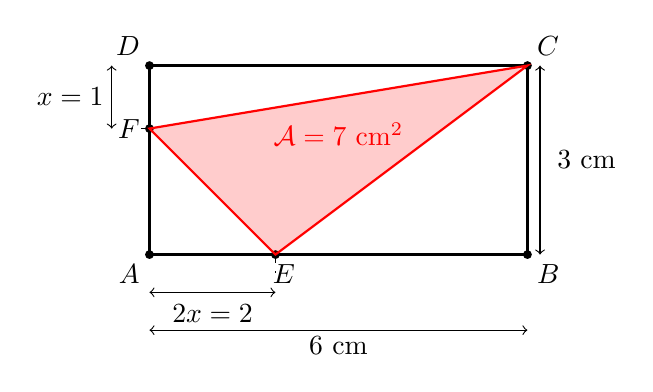
\begin{tikzpicture}[scale=0.8]
% Rectangle ABCD (6cm x 3cm)
\draw[thick] (0,0) rectangle (6,3);

% Points du rectangle
\fill (0,0) circle (2pt) node[below left] {$A$};
\fill (6,0) circle (2pt) node[below right] {$B$};
\fill (6,3) circle (2pt) node[above right] {$C$};
\fill (0,3) circle (2pt) node[above left] {$D$};

% Point E sur AB avec 2x=2 (x=1)
\fill (2,0) circle (2pt) node[below,xshift=3pt] {$E$};
\draw[dashed] (2,0) -- (2,-0.3);
\draw[<->] (0,-0.6) -- (2,-0.6);
\node[yshift=-10pt] at (1,-0.5) {$2x=2$};

% Point F sur AD avec DF=x=1
\fill (0,2) circle (2pt) node[left] {$F$};
\draw[dashed] (0,2) -- (-0.3,2);
\draw[<->] (-0.6,2) -- (-0.6,3);
\node[xshift=-15pt] at (-0.6,2.5) {$x=1$};

% Triangle FEC
\draw[red,thick] (0,2) -- (2,0) -- (6,3) -- cycle;
\fill[red,opacity=0.2] (0,2) -- (2,0) -- (6,3) -- cycle;

% Dimensions du rectangle
\draw[<->] (6.2,0) -- (6.2,3);
\node[xshift=10pt] at (6.5,1.5) {$3$ cm};
\draw[<->] (0,-1.2) -- (6,-1.2);
\node[yshift=-10pt] at (3,-1) {$6$ cm};

\node[red,yshift=15pt] at (3,1.25) {$\mathcal{A}=7$ cm$^2$};
\end{tikzpicture}

\tcbitem[title=Configuration avec aire minimale,halign=center]
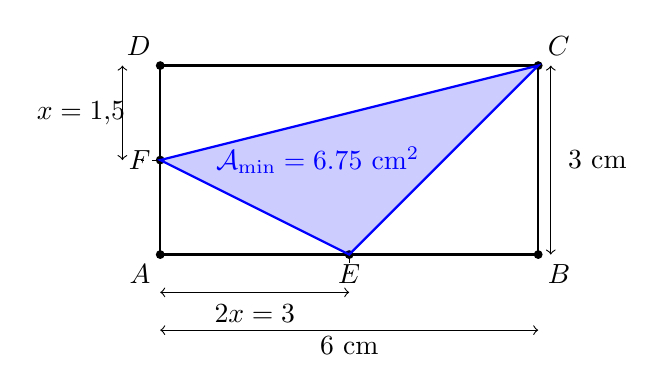
\begin{tikzpicture}[scale=0.8]
% Rectangle ABCD (6cm x 3cm)
\draw[thick] (0,0) rectangle (6,3);

% Points du rectangle
\fill (0,0) circle (2pt) node[below left] {$A$};
\fill (6,0) circle (2pt) node[below right] {$B$};
\fill (6,3) circle (2pt) node[above right] {$C$};
\fill (0,3) circle (2pt) node[above left] {$D$};

% Point E sur AB avec 2x=3 (x=1.5)
\fill (3,0) circle (2pt) node[below] {$E$};
\draw[dashed] (3,0) -- (3,-0.3);
\draw[<->] (0,-0.6) -- (3,-0.6);
\node[yshift=-10pt] at (1.5,-0.5) {$2x=3$};

% Point F sur AD avec DF=x=1.5
\fill (0,1.5) circle (2pt) node[left] {$F$};
\draw[dashed] (0,1.5) -- (-0.3,1.5);
\draw[<->] (-0.6,1.5) -- (-0.6,3);
\node[xshift=-15pt] at (-0.6,2.25) {$x=1{,}5$};

% Triangle FEC optimal
\draw[blue,thick] (0,1.5) -- (3,0) -- (6,3) -- cycle;
\fill[blue,opacity=0.2] (0,1.5) -- (3,0) -- (6,3) -- cycle;

% Dimensions du rectangle
\draw[<->] (6.2,0) -- (6.2,3);
\node[xshift=10pt] at (6.5,1.5) {$3$ cm};
\draw[<->] (0,-1.2) -- (6,-1.2);
\node[yshift=-10pt] at (3,-1) {$6$ cm};

\node[blue] at (2.5,1.5) {$\mathcal{A}_{\min}=\num{6.75}$ cm$^2$};
\end{tikzpicture}
\end{MultiColonnes}
\begin{tcbenumerate}[2]
\tcbitem[raster multicolumn=2] \textbf{Calcul de l'aire du triangle $FEC$ :}

\begin{MultiColonnes}{2}
\tcbitem $\text{Aire}_{FEC} = \text{Aire du rectangle} - \text{Aire des autres triangles}$

L'aire du rectangle $ABCD$ est : $6 \times 3 = 18$ cm$^2$ ; de plus :

\begin{MultiColonnes}{1}
    \tcbitem $\text{Aire}_{AFE} = \dfrac{1}{2} \times 2x \times (3-x) = x(3-x) =  {\color{blue}3x-x^2}$

    \tcbitem $\text{Aire}_{EBC} = \dfrac{1}{2} \times (6-2x) \times 3 = \dfrac{3}{2}(6-2x) =  {\color{red}9-3x}$

    \tcbitem $\text{Aire}_{FDC} = \dfrac{1}{2} \times x \times 6 =  {\color{defi}3x}$

\end{MultiColonnes}

\tcbitem Donc :
$\text{Aire}_{FEC} = 18 - \text{Aire}_{AFE} - \text{Aire}_{EBC} - \text{Aire}_{FDC}$

$= 18 -  {\color{blue}(3x-x^2)} - ( {\color{red}9-3x}) -  {\color{defi}3x}$

$= 18 - 3x + x^2 - 9 + 3x - 3x$

$= 18 - 9 + x^2 - 3x$

$= 9 + x^2 - 3x = x^2 - 3x + 9$
\end{MultiColonnes}



\tcbitem \textbf{Forme canonique et minimum :}

$A_{FEC}(x) = x^2 - 3x + 9$

Mettons sous forme canonique en utilisant la méthode du cours.

Pour $f(x) = ax^2 + bx + c$, on a : $\alpha = -\dfrac{b}{2a}$ et $\beta = f(\alpha)$

Ici : $a = 1$, $b = -3$, $c = 9$

$\alpha = -\dfrac{-3}{2 \times 1} = \dfrac{3}{2} = 1{,}5$

$\beta = f(1{,}5) = (1{,}5)^2 - 3 \times 1{,}5 + 9 = 2{,}25 - 4{,}5 + 9 = 6{,}75$

Donc : $A_{FEC}(x) = \left(x-\dfrac{3}{2}\right)^2 + \dfrac{27}{4}$


\tcbitem \textbf{Conclusion :}

Le minimum de $A_{FEC}(x)$ est atteint pour $\alpha = \dfrac{3}{2} = 1{,}5$.

Cette valeur appartient bien à $\intervalle{0}{3}$.

La valeur minimale de l'aire est $\beta = \dfrac{27}{4} = 6{,}75$ cm$^2$.

\textbf{Réponse :} L'aire du triangle $FEC$ est minimale pour $x = 1{,}5$ cm et vaut $6{,}75$ cm$^2$.
\end{tcbenumerate}

\end{bfEnv}



\end{document}